
We start by the first sentence of Bunge (2005) \cite{bung05}:
"The average temperature increase through Earth's
crust and mantle is called the geotherm. Its basic form is
assumed to consist of adiabatic regions where temperatures 
rise only slightly with depth, and of narrow thermal
boundary layers where temperatures increase rapidly
over a depth of a few hundred kilometers (Jeanloz and
Morris, 1986) \cite{jemo86}."

Before we look further at the equations behind this temperature profile, 
we must look at the basic assumption we make about
the type of convection taking place in the mantle:
layered convection vs. whole mantle convection, as
depicted here: 

\begin{center}
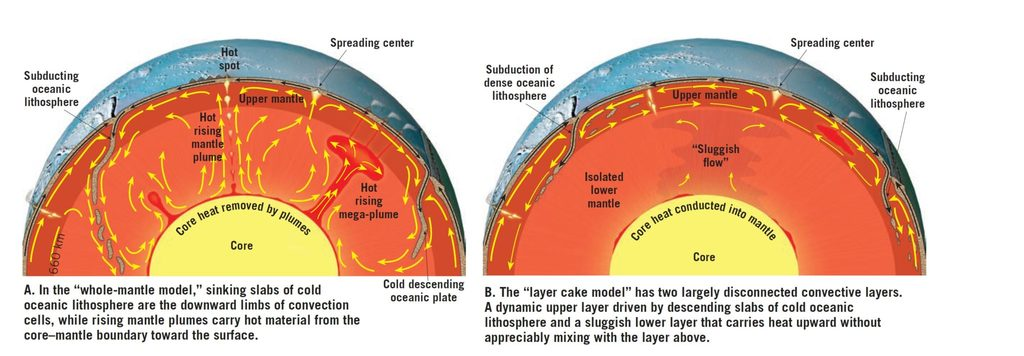
\includegraphics[width=12cm]{images/adiabatic/modes}\\
{\captionfont Taken from \url{https://geologyengineering.com/2020/05/mantle-convection/}}
\end{center}

\noindent Indeed, the type of convection is then expected to have an strong influence 
on the radial temperature profile: 

\begin{center}
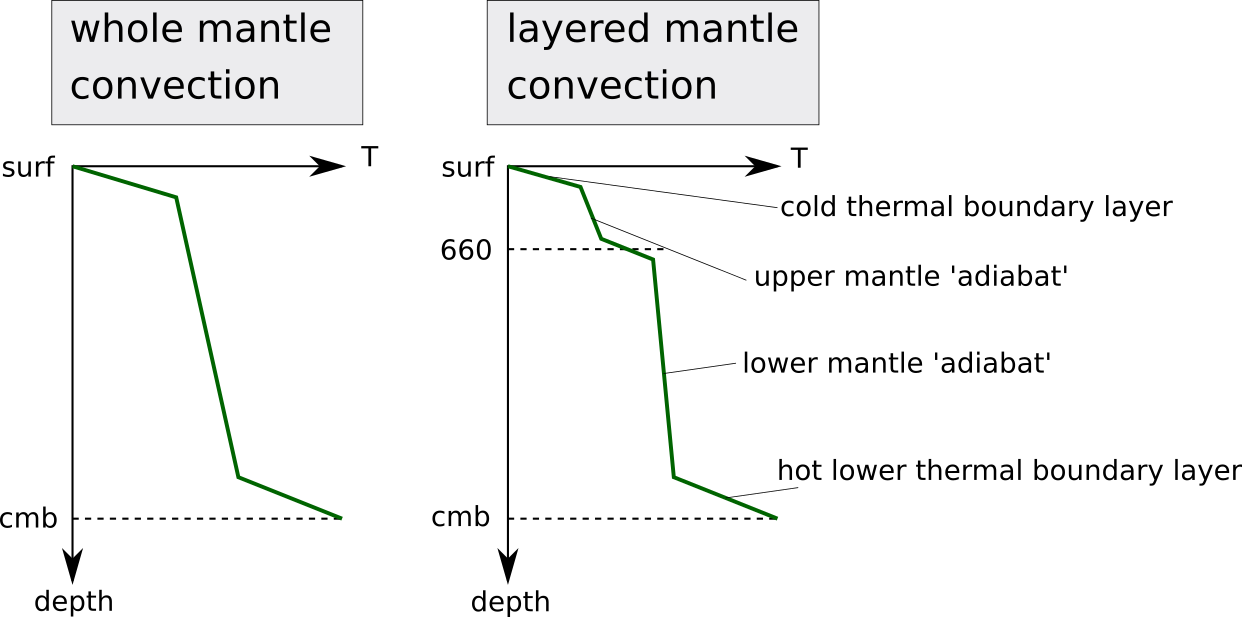
\includegraphics[width=10cm]{images/adiabatic/drawing.png}
\end{center}

This is also to be found in Poirier's book \cite{poirier}:
\begin{center}
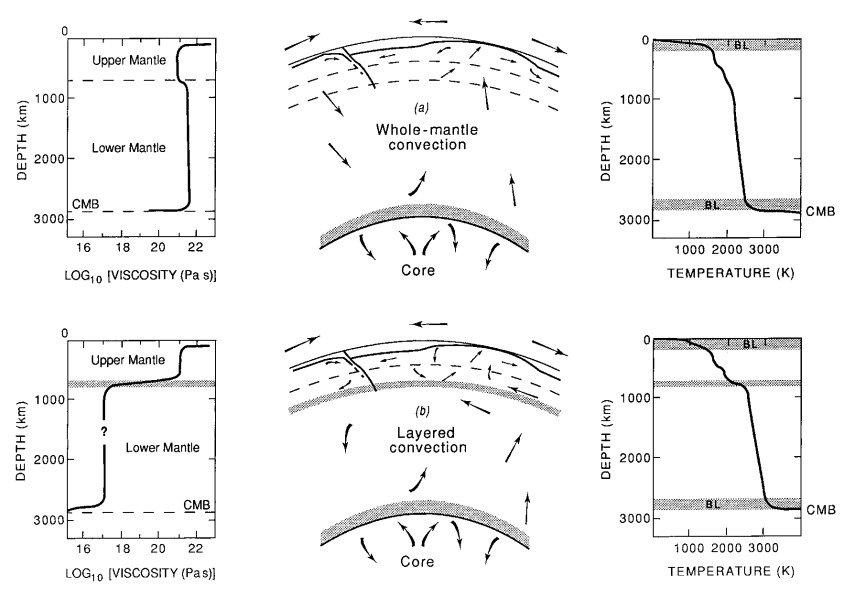
\includegraphics[width=11cm]{images/adiabatic/poirier}\\
{\captionfont Schematic diagrams of (a) whole-mantle and (b) layered convection
models, with corresponding temperature and viscosity profiles (after 
Peltier \& Jarvis (1982) \cite{peja82}.)}
\end{center}


The two-layered convection hypothesis relies essentially 
on the viscosity jump at the 660 discontinuity and seems 
to be generally accepted.
It also forms the basis of {\v{C}}adek \& van den Berg (1998) \cite{cava98}
in which the authors carry out an inversion to obtain 
radial profiles of temperature and viscosity in the Earth’s mantle
inferred from the geoid and lateral seismic structure:
\begin{center}
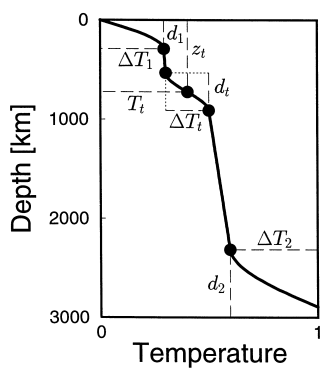
\includegraphics[width=6cm]{images/adiabatic/cava98a.png}
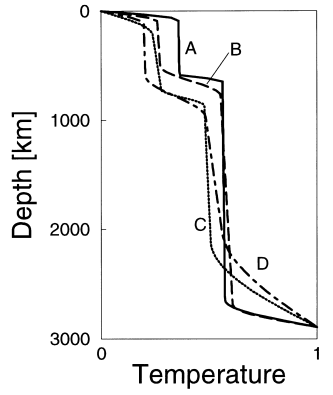
\includegraphics[width=5.5cm]{images/adiabatic/cava98b.png}\\
{\captionfont Taken from \cite{cava98}. 
Left: Parameterization of the geotherm used in the paper;
Right: Four model geotherms reducing the misfit by 70\%. The
differences between the models illustrate uncertainties of the
solution.}
\end{center}

More recently, Katsura et al (2010) \cite{kayy10} have constructed the following mantle temperature 
and temperature gradient profiles:

\begin{center}
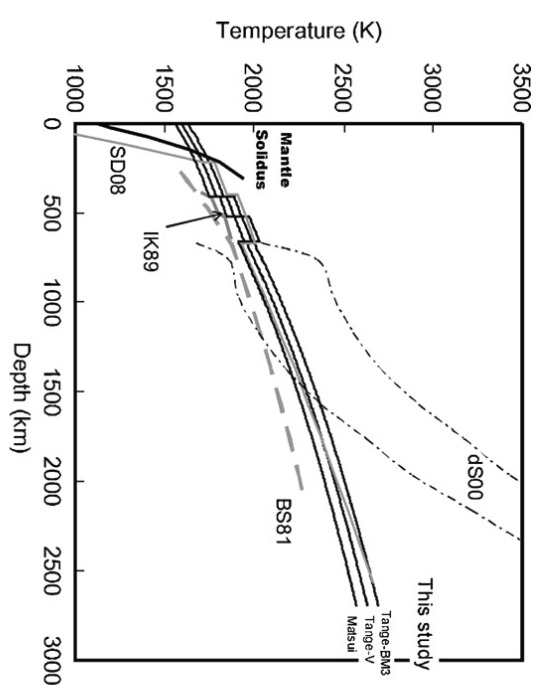
\includegraphics[width=6cm]{images/adiabatic/kayy10a}
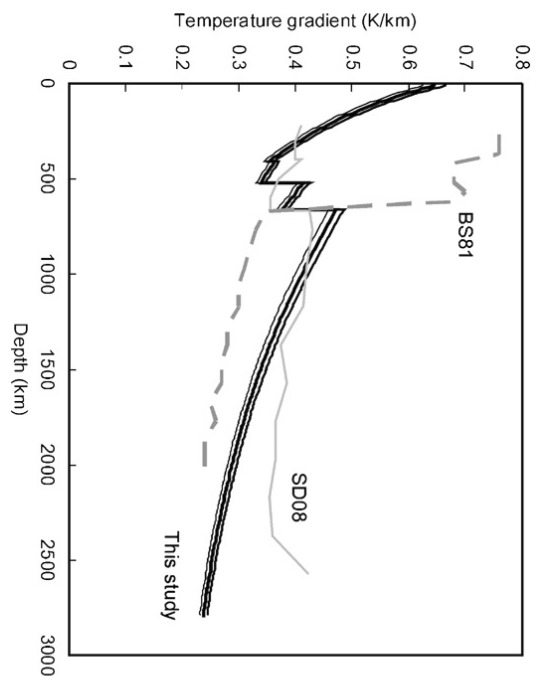
\includegraphics[width=6cm]{images/adiabatic/kayy10b}\\
{\captionfont Taken from Katsura et al (2010) \cite{kayy10}.
Left: The adiabatic temperature distributions in the mantle. The three solid lines
denote the temperature distributions proposed in this study using three different
pressure scales. Those proposed by the previous studies are shown for comparison
(BS81: Brown and Shankland, 1981; IK89: Ito and Katsura, 1989; dS00: da Silva et al.,
2000; SD08: Stacey and Davis, 2008). The mantle solidus proposed by Hirschmann
(2000) is also shown.
Right:
Adiabatic temperature gradient in the mantle. The adiabatic temperature gradient 
abruptly increases in association with the olivine–wadsleyite,
wadsleyite–ringwoodite, ringwoodite–perovskite + periclase transitions, as is the
case for the thermal expansion. The adiabatic temperature gradients given in the
previous studies are also shown for comparison (BS81: Brown and Shankland, 1981;
SD08: Stacey and Davis, 2008 \cite{stacey_davis}).
}
\end{center}


Prof. Steinberger was gracious to communicate to me the data of Steinberger \& Calderwood (2006) \cite{stca06}:
\begin{center}
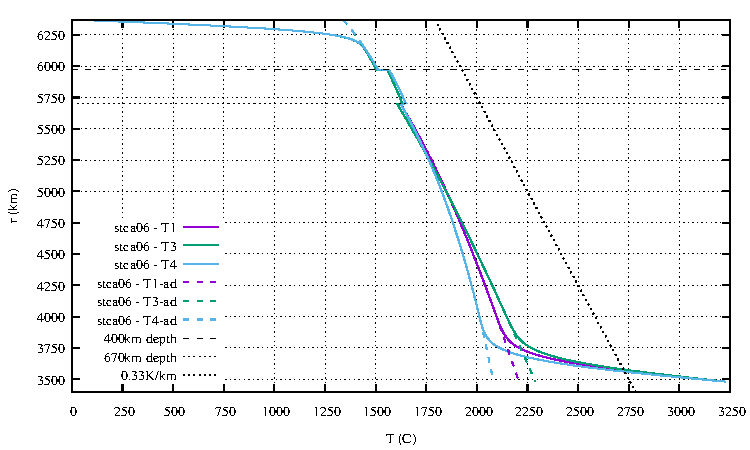
\includegraphics[width=8.5cm]{images/adiabatic/steinberger/Tprofile.pdf}
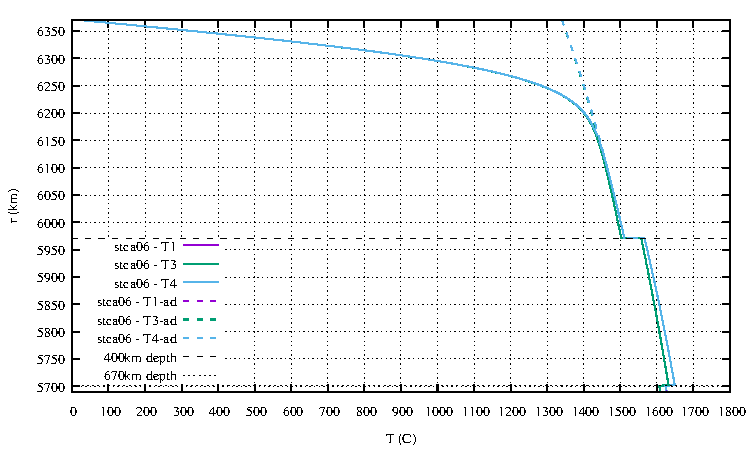
\includegraphics[width=8.5cm]{images/adiabatic/steinberger/Tprofile_upper.pdf}\\
{\captionfont Temperature profiles from Steinberger \& Calderwood \cite{stca06}.}
\end{center}

One can gather data from various papers and books and this yields the following 
figure\footnote{It must be said that finding actual data -not figures- is remarkably difficult.}:

\begin{center}
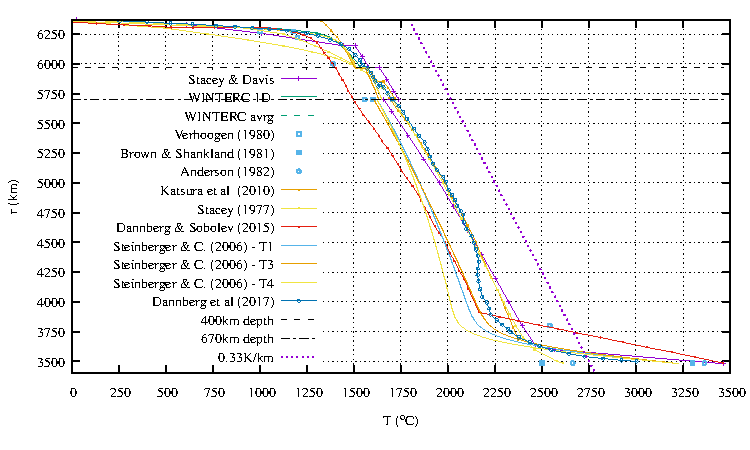
\includegraphics[width=8.5cm]{images/adiabatic/Tprofile.pdf}
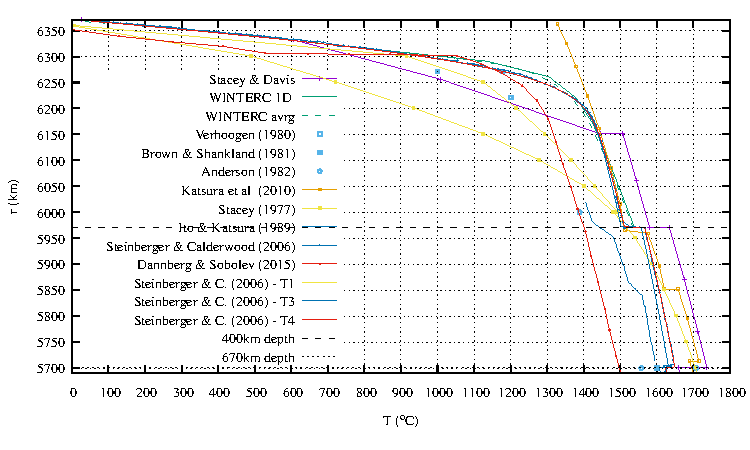
\includegraphics[width=8.5cm]{images/adiabatic/Tprofile_upper.pdf}\\
{\captionfont 
Note that the T values of Stacey (1977) \cite{stac77} inexplicably go to 540-550K at the surface. 
The value 545 has therefore been subtracted from the values in the paper. These then 
align remarquably well with those of Katsura et al.
}
\end{center}




We see that there is a remarkable agreement between many studies for the temperature down to 400km 
depth. Most show a step in the profile between 400 and 670km depth but the temperature at 670km
depth seems to be between 1650$\si{\celsius}$ and 1750$\si{\celsius}$.
Further down, the discrepancy between studies increases (effectively boiling down to 
the value of the adiabatic gradient). 100km above the CMB all studies seem to indicate a 
temperature of 2300-2400$\si{\celsius}$. Temperature values at the CMB differ a lot and 
as noted in Bull et al (2009) \cite{bumr09}: 
"Estimates of CMB temperature vary greatly. [...] 
We impose a surface temperature of 273 K and
investigate three CMB temperatures: 3000 K (consistent with
previous studies of this nature, e.g., Kellogg et al., 1999 \cite{kehv99}), 3950 K
(consistent with recent results on the double-crossing of Post-
Perovskite, e.g., Hernlund et al., 2005 \cite{hett05}; van der Hilst et al., 
2007 \cite{vadw07}; Alf\`e et al., 2002), and 4800 K (Knittle and Jeanloz, 1991). The 3950 K
temperature is the 'reference' temperature which we use for the
majority of cases."
The CMB temperature is set to $2900-3200\si{\celsius}$ in Fowler \cite{fowler}.


Also, oceanic plates being thinner than continental plates (alongside with different 
radiogenic decay and thermal properties) one can draw two representative mantle 
geotherms \cite{tusc}:

\begin{center}
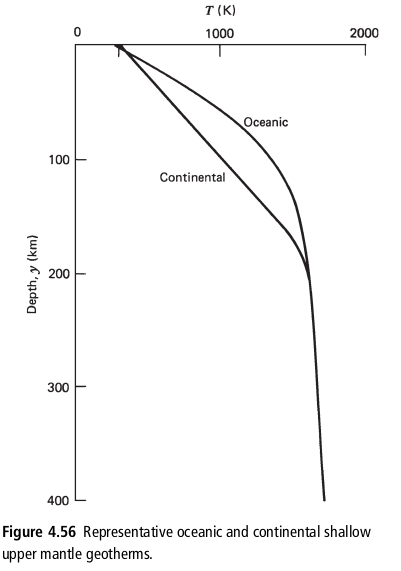
\includegraphics[width=4cm]{images/adiabatic/tusc.png}\\
{\captionfont Taken from Turcotte \& Schubert \cite{tusc}}
\end{center}




\newpage



[from ASPECT manual]



---------------------------------------------
\paragraph{Isentropic gradient}

The material properties also define the slope of the adiabat (the change in temperature with
pressure at constant entropy) at all pressures and temperatures. Using the cyclic relation,
we can define this slope in terms of partial differentials of the entropy with respect to pressure
and temperature:
\begin{eqnarray}
\left( \frac{\partial T}{\partial p} \right)_{S} 
&=& - \left( \frac{\partial T}{\partial S} \right)_{p} \left( \frac{\partial S}{\partial p} \right)_{T} \\
&=& - \left( \frac{T}{C_p} \right) \left( - \frac{\alpha}{\rho} \right) \\
&=& \frac{\alpha T}{\rho C_p} \label{eq:mm_isentropic_gradient}
\end{eqnarray}
This expression does not pose a constraint on the material properties, but in order to be 
self-consistent, the adiabat must be computed following this relation.

For complex material models, obtaining analytical functions which obey all these relations
may be a non-trivial exercise. Furthermore, it is often not immediately clear when a
given formulation is thermodynamically inconsistent. Indeed, both the
thermodynamic and the geodynamic literature contain many equations of
state and material parameterizations which do not obey these 
relations! This may not invalidate the results obtained with these 
models, but it is a point worth keeping in mind as the geodynamics
community moves to more complicated and more realistic parameterizations.

\emph{A final note of warning: Some compressible formulations in \aspect{}
  (Section~\ref{sec:mass-conservation-approximation}) use the isothermal compressibility,
  while others use the isentropic compressibility. Fully self-consistent material models must
  either specify what approximation of the compressible equations they are consistent with
  (see Section~\ref{sec:approximate-equations}), or have a switch so that they use the correct
  compressibility for each of the different approximations. The conversion between isothermal
  and isentropic compressibilities is given in~\eqref{eq:mm_isentropic_compressibility}.}

--------------------------------------------------

\paragraph{Initial conditions and the adiabatic pressure/temperature}

The thermo-mechanically coupled (Navier-)Stokes 
equations require us to
pose initial conditions for the temperature
Note that the equations
themselves do not require that initial conditions are specified for
the velocity and pressure variables (since there are no time
derivatives on these variables in the model).

Nevertheless, a nonlinear solver will have difficulty converging to
the correct solution if we start with a completely unphysical pressure
for models in which coefficients such as density $\rho$ and viscosity
$\eta$ depend on the pressure and temperature. To this end, \aspect{}
uses pressure and temperature fields $p_{\textrm{ad}}(z),
T_{\textrm{ad}}(z)$ computed in the adiabatic conditions model
(see Section~\ref{parameters:Adiabatic_20conditions_20model}).
By default, these fields satisfy adiabatic conditions:
\begin{align}
\rho C_p \frac{\textrm{d}}{\textrm{d}z} T_{\textrm{ad}}(z)
&=
\frac{\partial\rho}{\partial T} T_{\textrm{ad}}(z) g_z,
\\
\frac{\textrm{d}}{\textrm{d}z} p_{\textrm{ad}}(z)
&=
\rho g_z,
\end{align}
where strictly speaking $g_z$ is the magnitude of the vertical
component of the gravity vector field, but in practice we take the
magnitude of the entire gravity vector.

These equations can be integrated numerically starting at $z=0$, using
the depth dependent gravity field and values of the coefficients
$\rho=\rho(p,T,z), C_p=C_p(p,T,z)$. As starting conditions at $z=0$ we
choose a pressure $p_{\textrm{ad}}(0)$ equal to the average surface
pressure (often chosen to be zero, see Section~\ref{sec:pressure}),
and an adiabatic surface temperature $T_{\textrm{ad}}(0)$ that is
also selected in the input parameter file.
%\index[prmindex]{Adiabatic surface temperature}
%\index[prmindexfull]{Adiabatic surface temperature}

\note{The adiabatic surface temperature is often chosen significantly
  higher than the actual surface temperature. For example, on earth,
  the actual surface temperature is on the order of 290 K, whereas a
  reasonable adiabatic surface temperature is maybe 1600 K. The reason
  is that the bulk of the mantle is more or less in thermal equilibrium
  with a thermal profile that corresponds to the latter temperature,
  whereas the very low actual surface temperature and the very high
  bottom temperature at the core-mantle boundary simply induce a
  thermal boundary layer. Since the temperature and pressure profile
  we compute using the equations above are simply meant to be good
  starting points for nonlinear solvers, it is important to choose
  this profile in such a way that it covers most of the mantle well;
  choosing an adiabatic surface temperature of 290 K would yield a
  temperature and pressure profile that is wrong almost throughout the
  entire mantle.}

For instance, let us consider $\alpha=3\cdot 10^{-5}$, 
$g_z=10$, $C_p=1250$, $\rho=\rho_0(1-\alpha (T-T_0)$ so that 
$\frac{\partial\rho}{\partial T} = -\alpha \rho_0$ 
with $\rho_0=3300$.

Then we must solve the following equation
\[
\rho_0(1-\alpha(T-T_0)) C_p \frac{\textrm{d}T}{\textrm{d}z} 
=
- \alpha T^2  g_z
\]

----------------------------------

In Verhoogen (1951) \cite{verh51}:
As is well known, the adiabatic gradient may be written as
\[
\frac{dT}{dP} = \alpha T /\rho C_p
\]
If hydrostatic equilibrium is assumed, the pressure varies with depth $h$ as 
$dP = \rho g dh$, so that
\[
\frac{d \ln T}{dh} = \frac{\alpha g}{C_p}
\]
from which the temperature $T$ at any depth $h$ may be computed as a function of the temperature
at any assigned depth if the ratio $\alpha/C_p$ 
is known at all depths ($g$, the acceleration of gravity, will
be taken as constant in the mantle).

----------------------------------


----------------------------------

From DyMaLi: In the interior of a convecting medium temperatures follow an adiabatic profile. 
At the top and bottom of a convecting layer thermal boundary layers with large thermal gradients form. 
The interior is thermally well mixed and therefore essentially isothermal, with a slight increase 
of temperatures with depth due to the effect of pressure.
For example in the Earth’s mantle the geothermal gradient ∂T /∂z is about 20C/km near the 
surface and about 0.3C/km in the interior of the mantle. This small gradient in the 
interior is the adiabatic gradient. If a small
volume of material is moved to shallower depth is experiences a slight increase in volume 
due to the decreasing pressure and associated with this a slight decrease in temperature. 
This change in temperature is the adiabatic temperature change.

The adiabatic gradient can be determined from the thermodynamics relation between entropy per unit mass S,
temperature T, and pressure P:
\[
dS = \left( \frac{dS}{dT}\right)_P dT +  \left( \frac{dS}{dP}\right)_T dP
=
\frac{C_p }{T} dT - \frac{\alpha}{\rho} dP
\]
In case of a reversible adiabatic process the entropy change is zero, and so the adiabatic gradient is:
\[
\left( \frac{dT}{dP}\right)_S = \frac{\alpha T}{\rho C_p} 
\]
The gradient can also be expressed in terms of depth, remembering that $d p = \rho gdz$ 
in a hydrostatic fluid:
\[
\left( \frac{dT}{dz}\right)_S = \frac{\alpha g T}{C_p} 
\]
Thus to determine the adiabatic gradient one needs values of $\alpha$ 
and $C_p$ with depth. These are obtained from laboratory experiments.

One also needs an estimate of density as a function of depth, which is generally determined
from seismology. 
Integration of the adiabatic gradient in terms of pressure then gives
temperature as a function of pressure. 
Temperature as a function of depth is obtained by integrating the density
distribution to obtain g as a function of depth.

not finished
----------------------------------

Vol07\_02

This adiabaticity hypothesis should, however, not
be taken too literally (Jeanloz and Morris, 1987 \cite{jemo87}). In
most numerical simulations, the resulting averaged
geotherm can be far (a few hundred kelvins) from
adiabatic (Bunge et al., 2001 \cite{burm01}). First, radioactive 
heating, dissipation, and diffusion are never totally
negligible, second, even if each fluid parcel follows
its own adiabatic geotherm, the average geotherm
may not correspond to any particular adiabat.



----------------------------------
From Steinberger oct 26th, 2020:

Yes, I think the temperature below the lithosphere is still fairly well-constrained, based on magmas produced on mid-oceanic ridges (away from plumes) if one takes these as representative. Regarding Dannberg and Sobolev (not Solomatov!) I don't know why it is lower. In their supplementary figures, the extrapolation to the surface is actually ~1250 K, not 1250°C, which is even less. Perhaps best to directly ask Juliane about this.

How the temperature increases with depth is more uncertain; the temperature gradient is often taken as adiabatic; that's what I also assumed in the 2006 paper, then it is defined by a ordinary differential equation (eq. 12 in that paper). I think the main uncertainty is the thermal expansivity. In my model, it strongly decreases with depth, I guess that is why my models have a lower temperature in the lower mantle than other models. I think that strong decrease in expansivity is still the consensus, but I didn't closely follow the literature recently. But the temperature gradient between the thermal boundary layers may actually be subadiabatic, hence even lower, due to cold slabs sinking to and accumulating above the CMB, and hot plume material feeding into the asthenosphere, below the lithosphere. So, yes, I would say the difference in the deep mantle (if not more) reflects the current state in the community.

And I think the uncertainites of CMB temperature are even larger. And I would of course be happy if you host my data on a public github repo. Just for the viscosity profile, there should be some explanation given that it shouldn't necessarily be taken "at face value" but that (like in the 2006 paper) it is possible to multiply different parts of the profile with different "scaling viscosities".

----------------------------------

\Literature: 
{\it On the thermal gradient in the Earth’s deep interior}, Tirone (2016) \cite{tiro16} \\
{\it Is the mantle geotherm subadiabatic}, Jeanloz \& Morris (1987) \cite{jemo87} \\
{\it Mantle convection, the asthenosphere, and Earth's thermal history} King (2015) \cite{king15}\\

check section 7.7 in Fowler !

boundary layer jape82

evolution shpe79
